\section{Qu'est ce qui ne fonctionne pas ?}

On réalise les expériences suivantes avec deux lampes $L_1$, $L_2$ et deux piles $P_1$ et $P_2$. Une lampe est défectueuse et une pile est usée. La lampe brille uniquement dans l'expérience A.

\begin{center}
	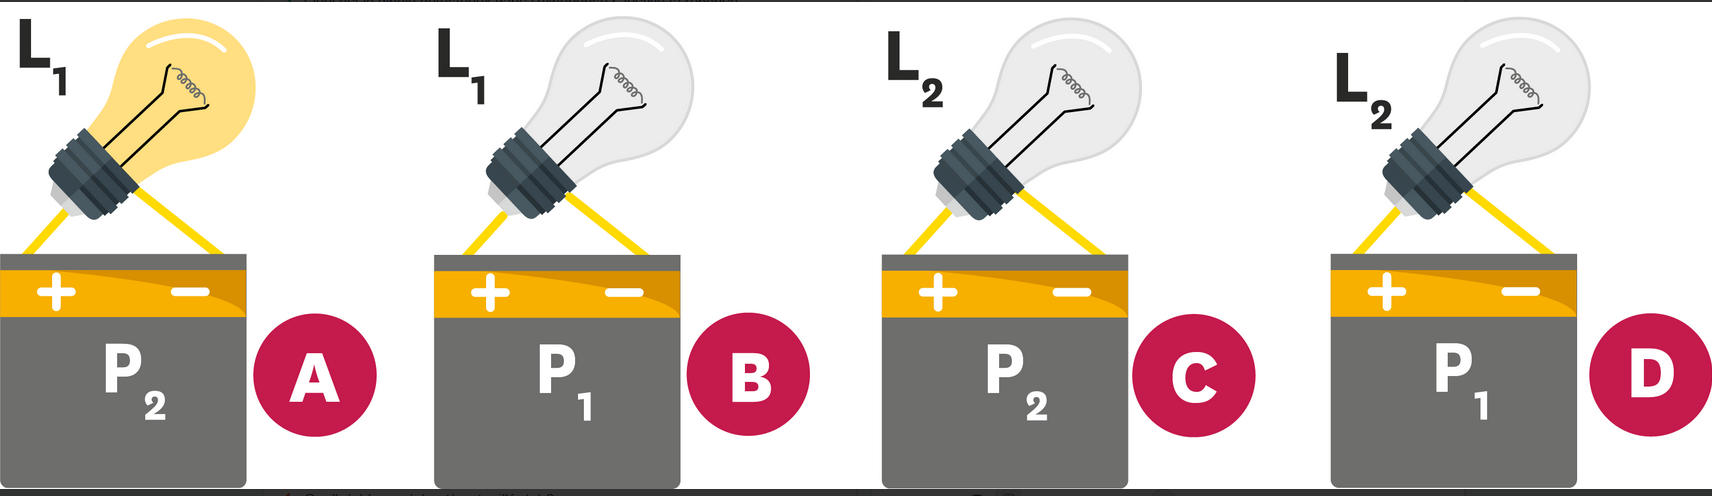
\includegraphics[scale=0.3]{img/lampes_piles}
\end{center}

\begin{questions}
	\question Dans l'expérience $A$, les dipôles sont-ils en bon état ? Expliquer la réponse en les nommant.
	
	\question Dans l'expérience $B$, quel est le dipôle défectueux ?
	
	\question Dans l'expérience $C$, quel est le dipôle défectueux ?
	
	Pour résumer :
	\question Quelle lampe est grillée ?
	
	\question Quelle pile est usagée ?
	
	\question Pour quelle(s) raison(s) la lampe $L_2$ ne brille pas dans l'expérience $D$ ?
	\end{questions}

